\documentclass[12pt, a4paper]{article}
    
\usepackage{homework}
\usepackage{amsmath}				% For Math
\usepackage{fancyhdr}				% For fancy header/footer
\usepackage{graphicx}				% For including figure/image
\usepackage{cancel}					% To use the slash to cancel out stuff in work
\usepackage{multirow}

%%%%%%%%%%%%%%%%%%%%%%
% Set up fancy header/footer
\pagestyle{fancy}
\setlength{\headheight}{42pt}
\fancyhead[LO,L]{Name: Yu Ching Hei\\SID: 1155193237\\email: chyu2@cse.cuhk.edu.hk}
\fancyhead[CO,C]{}
\fancyhead[RO,R]{CENG3420 Computer Organization and Design\\Lab 2.1\\Date: \today}
\fancyfoot[LO,L]{}
\fancyfoot[CO,C]{}
\fancyfoot[RO,R]{Page \thepage}
\renewcommand{\headrulewidth}{0.4pt}
\renewcommand{\footrulewidth}{0.4pt}
%%%%%%%%%%%%%%%%%%%%%%

\begin{document}
\begin{qNoMark}
Implement an RISCV-LC Assembler. 
\end{qNoMark}

\begin{ans}
\\\indent In this lab, we are going to complete some of the instructions in the \texttt{asm.c} file. 
There are few main points to mark and it is going to be stated in this lab report. 
In the following part, I am going to demonstrate how I complete this lab. 

For integer R-I Instructions, they have the same pattern as \texttt{ADDI} instruction, which is I-Type instruction. 
So basically I can just modify the \texttt{ADDI} instruction to add corresponding funct3(bit12-14) to the binary output and 
change some of the argument parsing of \texttt{arg3} for the shift functions like \texttt{SLLI, SRLI, SRAI} instructions. Here 
is one of my implementations of assembling integer R-I Instructions instruction, this case using \texttt{SRAI} instruction. 
\begin{code}
//other cases
else if (is_opcode(opcode) == SRAI) {
    binary = (0x04 << 2) + 0x03;
    binary += (reg_to_num(arg1, line_no) << 7);
    binary += (0x05 << 12);
    binary += (reg_to_num(arg2, line_no) << 15);
    binary += (lower5bit(arg3, line_no) << 20);
    binary += (0x010 << 26);
}
//continue on other cases
\end{code}
Line 9 adds the funct3 to the binary, line 11 extract the lower 5 bits of the immediate which stands for the number of bits to be 
shifted, and line 11 is adding value to binary to define the funct7 of the corresponding instruction. 

For Integer R-R operations, they have the same pattern as \texttt{ADD} instruction, which is R-Type instruction. 
So basically I can just modify the \texttt{ADD} instruction to add corresponding funct3(bit12-14) and funct7(bit25-31) to the binary output. 
Here is one of my implementations of assembling integer R-R Instructions instruction, this case using \texttt{SRA} instruction. 
\begin{code}
//other cases
else if (is_opcode(opcode) == SRA) {
    /* Lab2-1 assignment */
    binary = (0x0C << 2) + 0x03;
    binary += (reg_to_num(arg1, line_no) << 7);
    binary += (0x05 << 12);
    binary += (reg_to_num(arg2, line_no) << 15);
    binary += (reg_to_num(arg3, line_no) << 20);
    binary += (0x020 << 25);
}
//continue other cases
\end{code}
Line 6 add corresponding funct3 to the binary, line 7 and 8 handle corresponding register arguments, line 9 add corresponding funct7 to the binary. 
\pagebreak

For \texttt{JALR} instruction, it uses I-Type format. So the assembling format is similar to \texttt{ADDI} instruction. 
Since \texttt{JALR} have only 2 arguments, and the arg2 contains both the offset immediate and the register, we have to use the function
\texttt{parse\_regs\_indirect\_addr()} to separate the arg2. Then put the corresponding part into the the binary. 

\begin{code}
//other cases
else if (is_opcode(opcode) == JALR) {
    binary = (0x019 << 2) + 0x03;
    binary += (reg_to_num(arg1, line_no) << 7);
    binary += (reg_to_num(parse_regs_indirect_addr(arg2, line_no)->reg, line_no) << 15);
    binary += ((parse_regs_indirect_addr(arg2, line_no)->imm) << 20);
}
//continue other cases
\end{code}

For \texttt{JAL} instruction, it uses special J-Type format. So the assembling logic is different to \texttt{JALR} instruction. 

\begin{code}
//other cases
else if (is_opcode(opcode) == JAL) {
    binary = (0x01b << 2) + 0x03;
    binary += (reg_to_num(arg1, line_no) << 7);
    int val = handle_label_or_imm(line_no, arg2, label_table, number_of_labels);
    int offset = val - addr;
    binary += ((offset & 0x100000) << (31 - 20)); //bit20
    binary += ((offset & 0x7FE) << 20); //bit10:1 
    binary += ((offset & 0b100000000000) << (20 - 11)); //bit11
    binary += ((offset & 0xFF000)); //bit19:12
}
//continue other cases
\end{code}
Since \texttt{JAL} have special implementation in the 20-bit jump immediate, masking and careful shifting is needed to put the immediate in the correct position. \\
bit20 of the immediate only need to shift (31 - 20) in order to be in the bit31 of the instruction. \\
bit10:1 is shifted to left 20 in order to align the first bit to bit21. \\
bit11 is masked separately then shifted by (20-11)bit to place at bit20. \\
bit19:12 are of the same position of the insturction so no shifting is needed. 

For conditional branches, they are in B-Type format, which requires careful masking and shifting as well. 
Since example is given, the parsing and shifting of immediate is done for us so all we need is just to modify the implementation 
and add the funct3 to the instructions to differ them from each other. 

For Load Instructions, they implement I-Type formatting. However, they only take 2 arguments so we have to separate the offset immediate and the register 
from arg2 by calling the \texttt{parse\_regs\_indirect\_addr()} and carefully put the register into position of rd and immediate respectively. Since example is given for the 
\texttt{LB} instruction, so all we need to do is to add the funct3 to the binary that differs from each other branch fucntions. 

For Store Instructions, they implement specail S-Type formatting. They only take 2 arguments so we have to separate the offset immediate and the register 
from arg2 by calling the \texttt{parse\_regs\_indirect\_addr()} and put them into correct position. 
And since they have similar structure as branch instructions execpt the immediate part, we only need to modify the position of immediate. 
\end{ans}
\pagebreak
The following are the screenshots of the lab results. 
\begin{figure}[H]
    \caption{make validate result}
    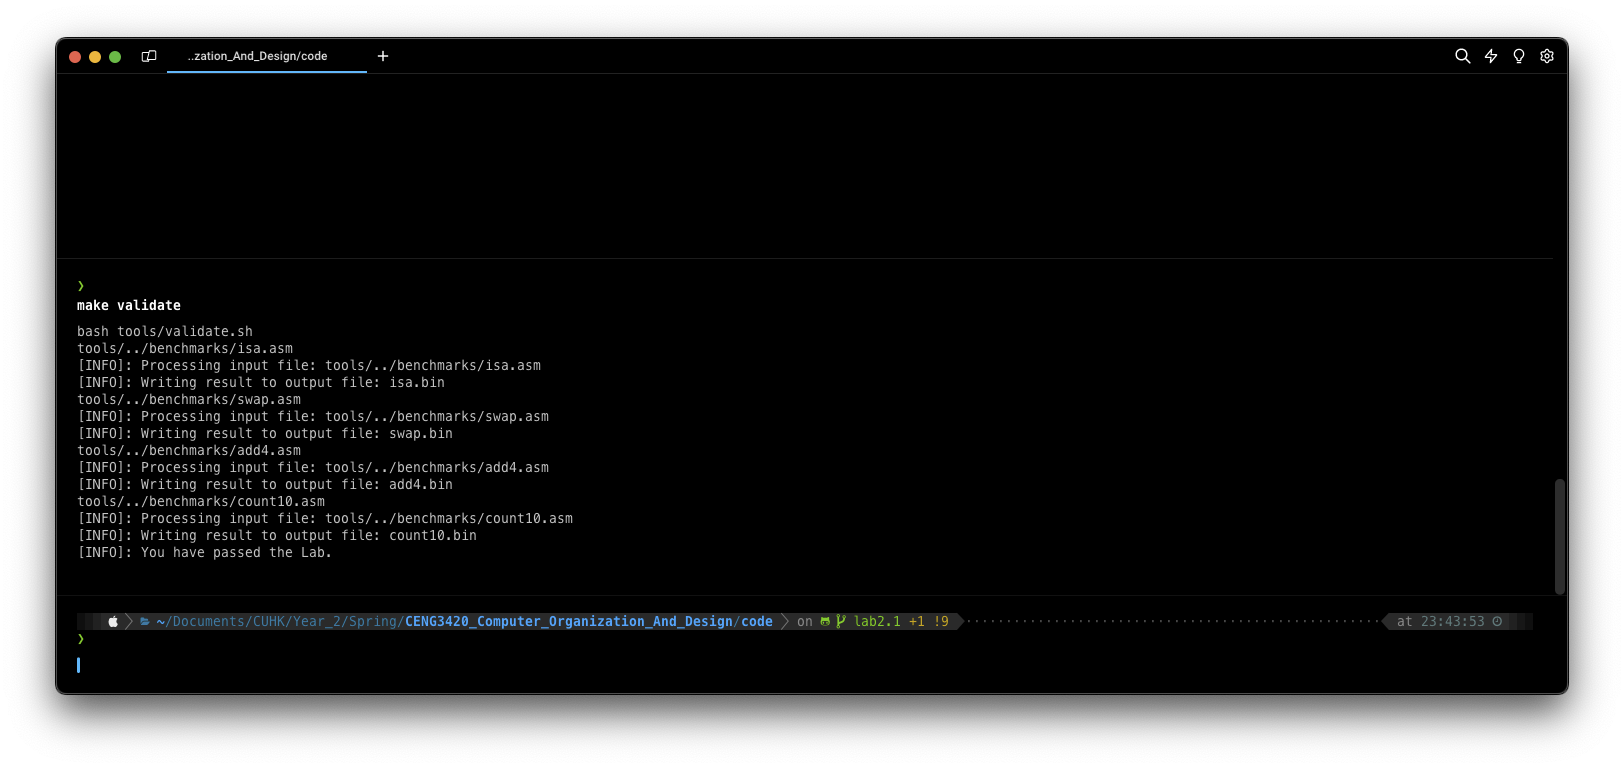
\includegraphics[width=1\linewidth]{../figs/validate.png}
\end{figure}

The following screenshots are the comparison of suggested answer(Left) and my output(Right). No highlighting means no different. 
\begin{figure}[H]
    \caption{add4.bin}
    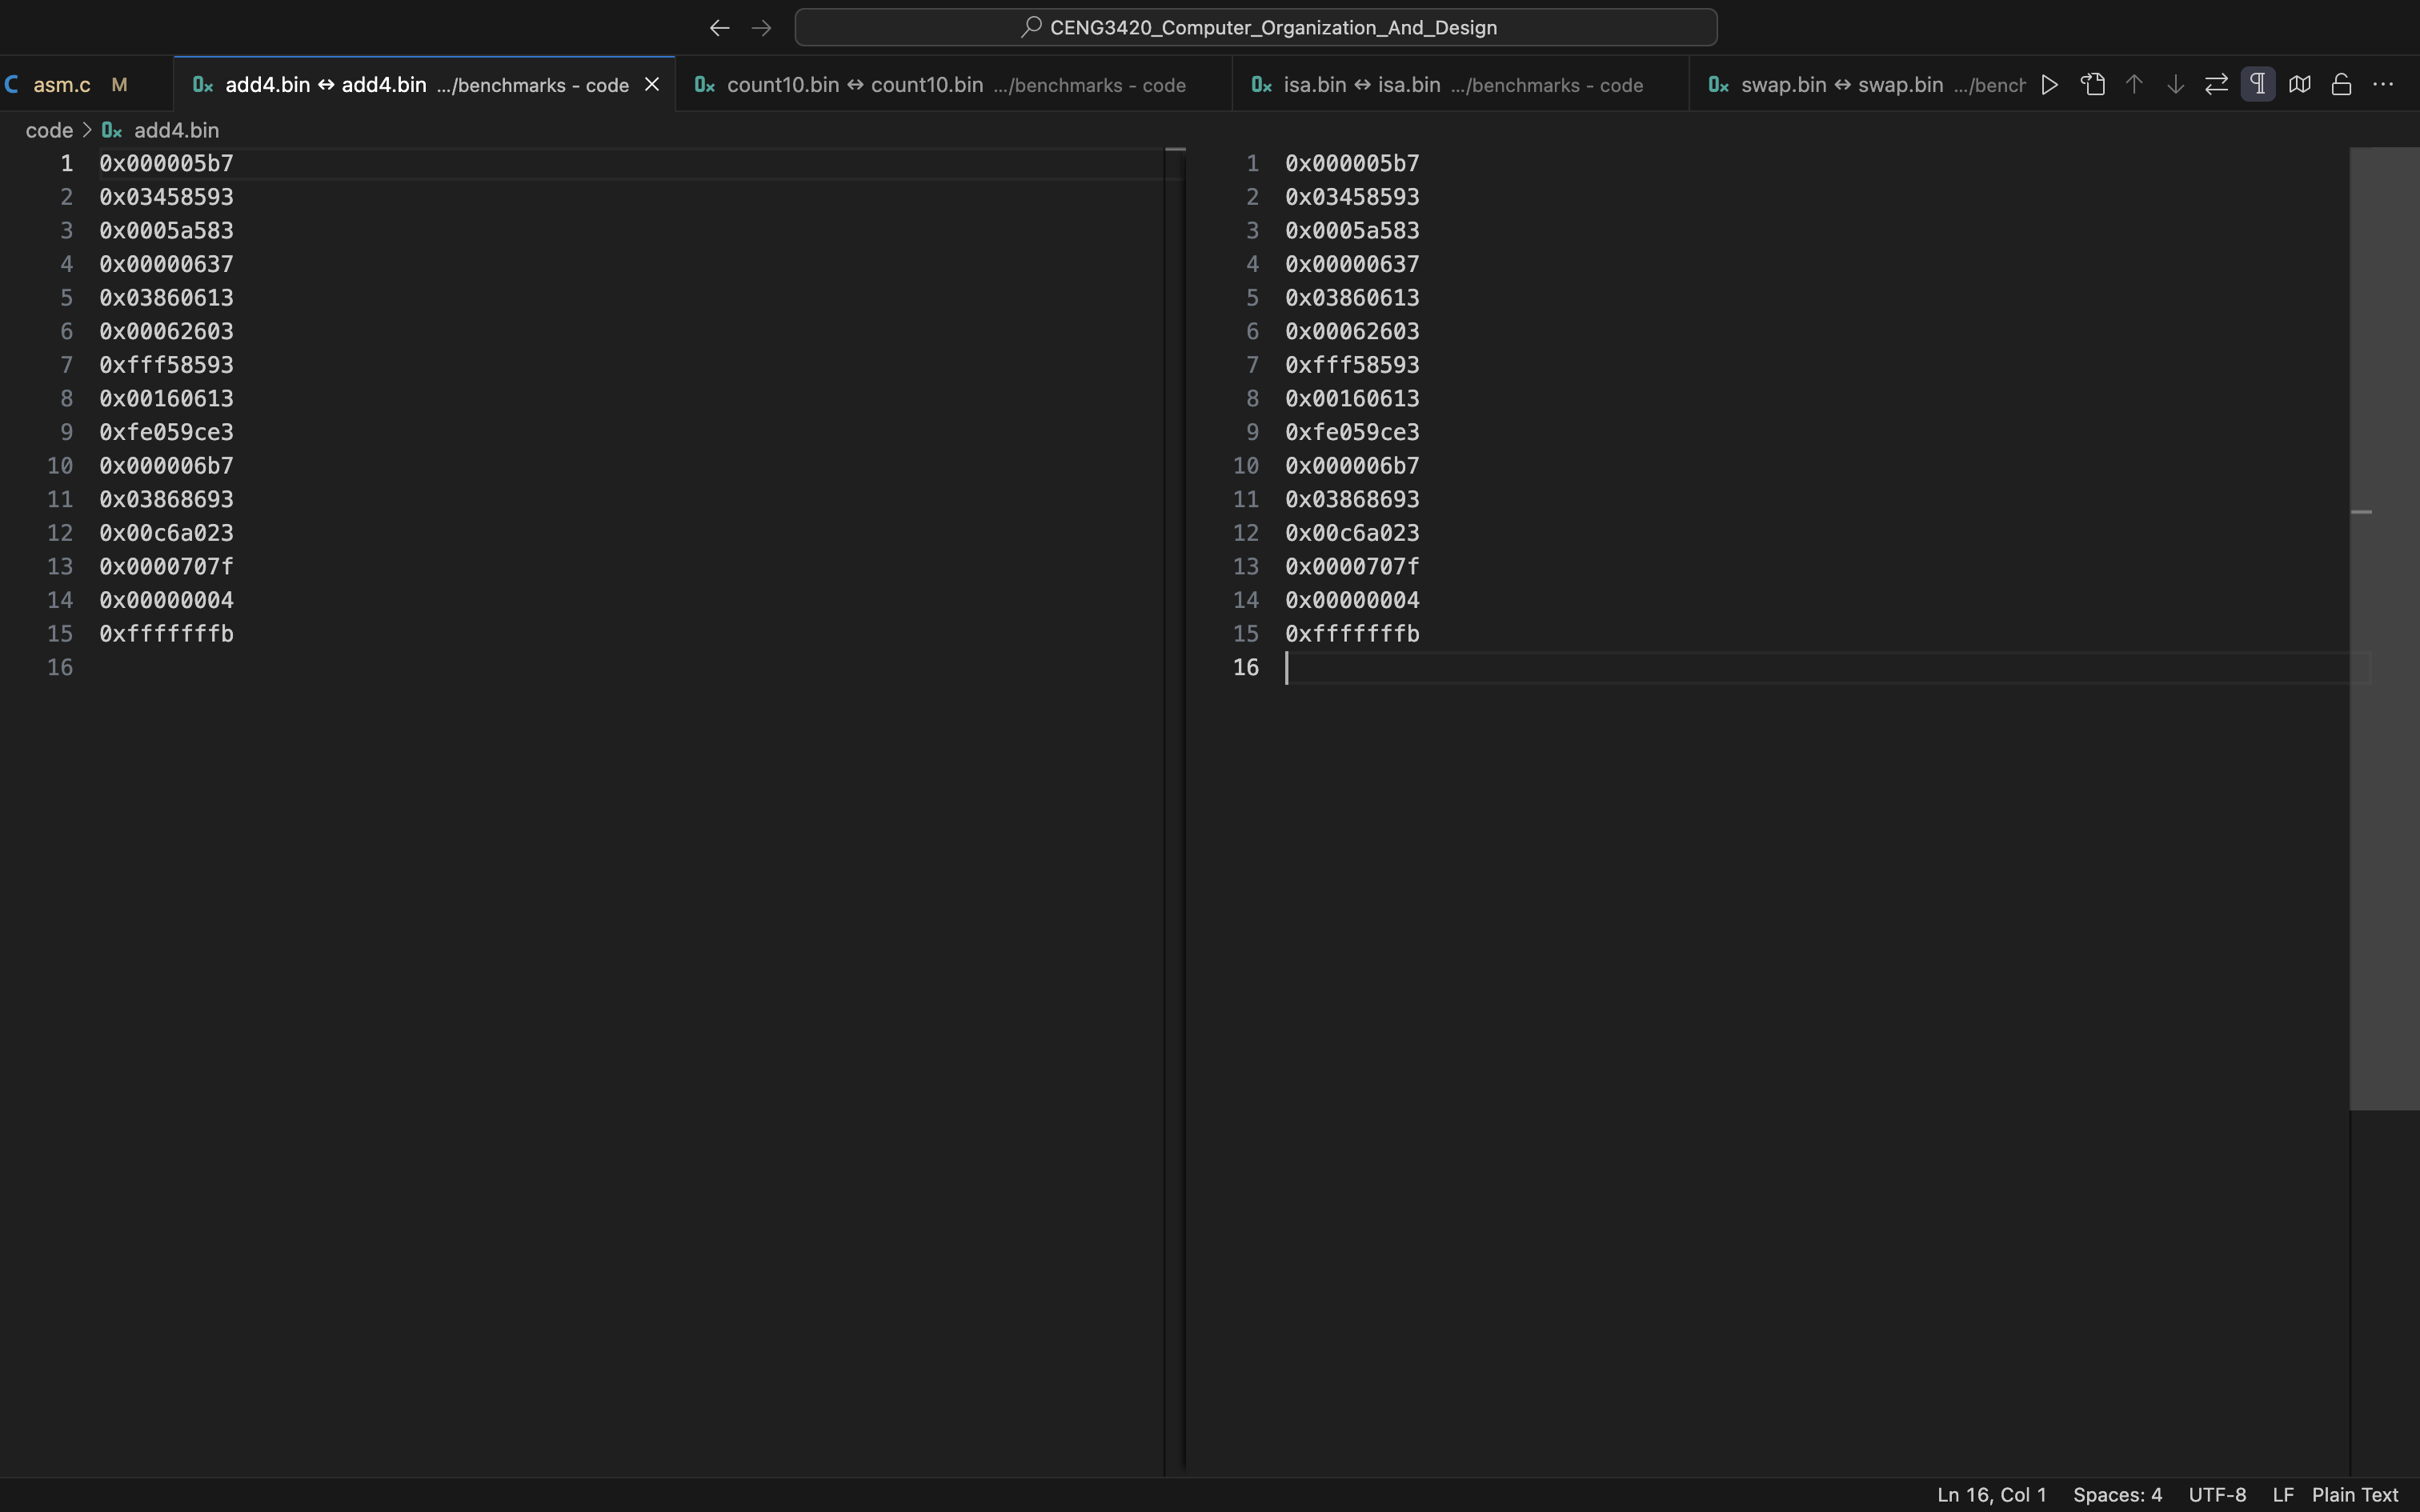
\includegraphics[width=1\linewidth]{../figs/add4.png}
\end{figure}

\begin{figure}[H]
    \caption{count10.bin}
    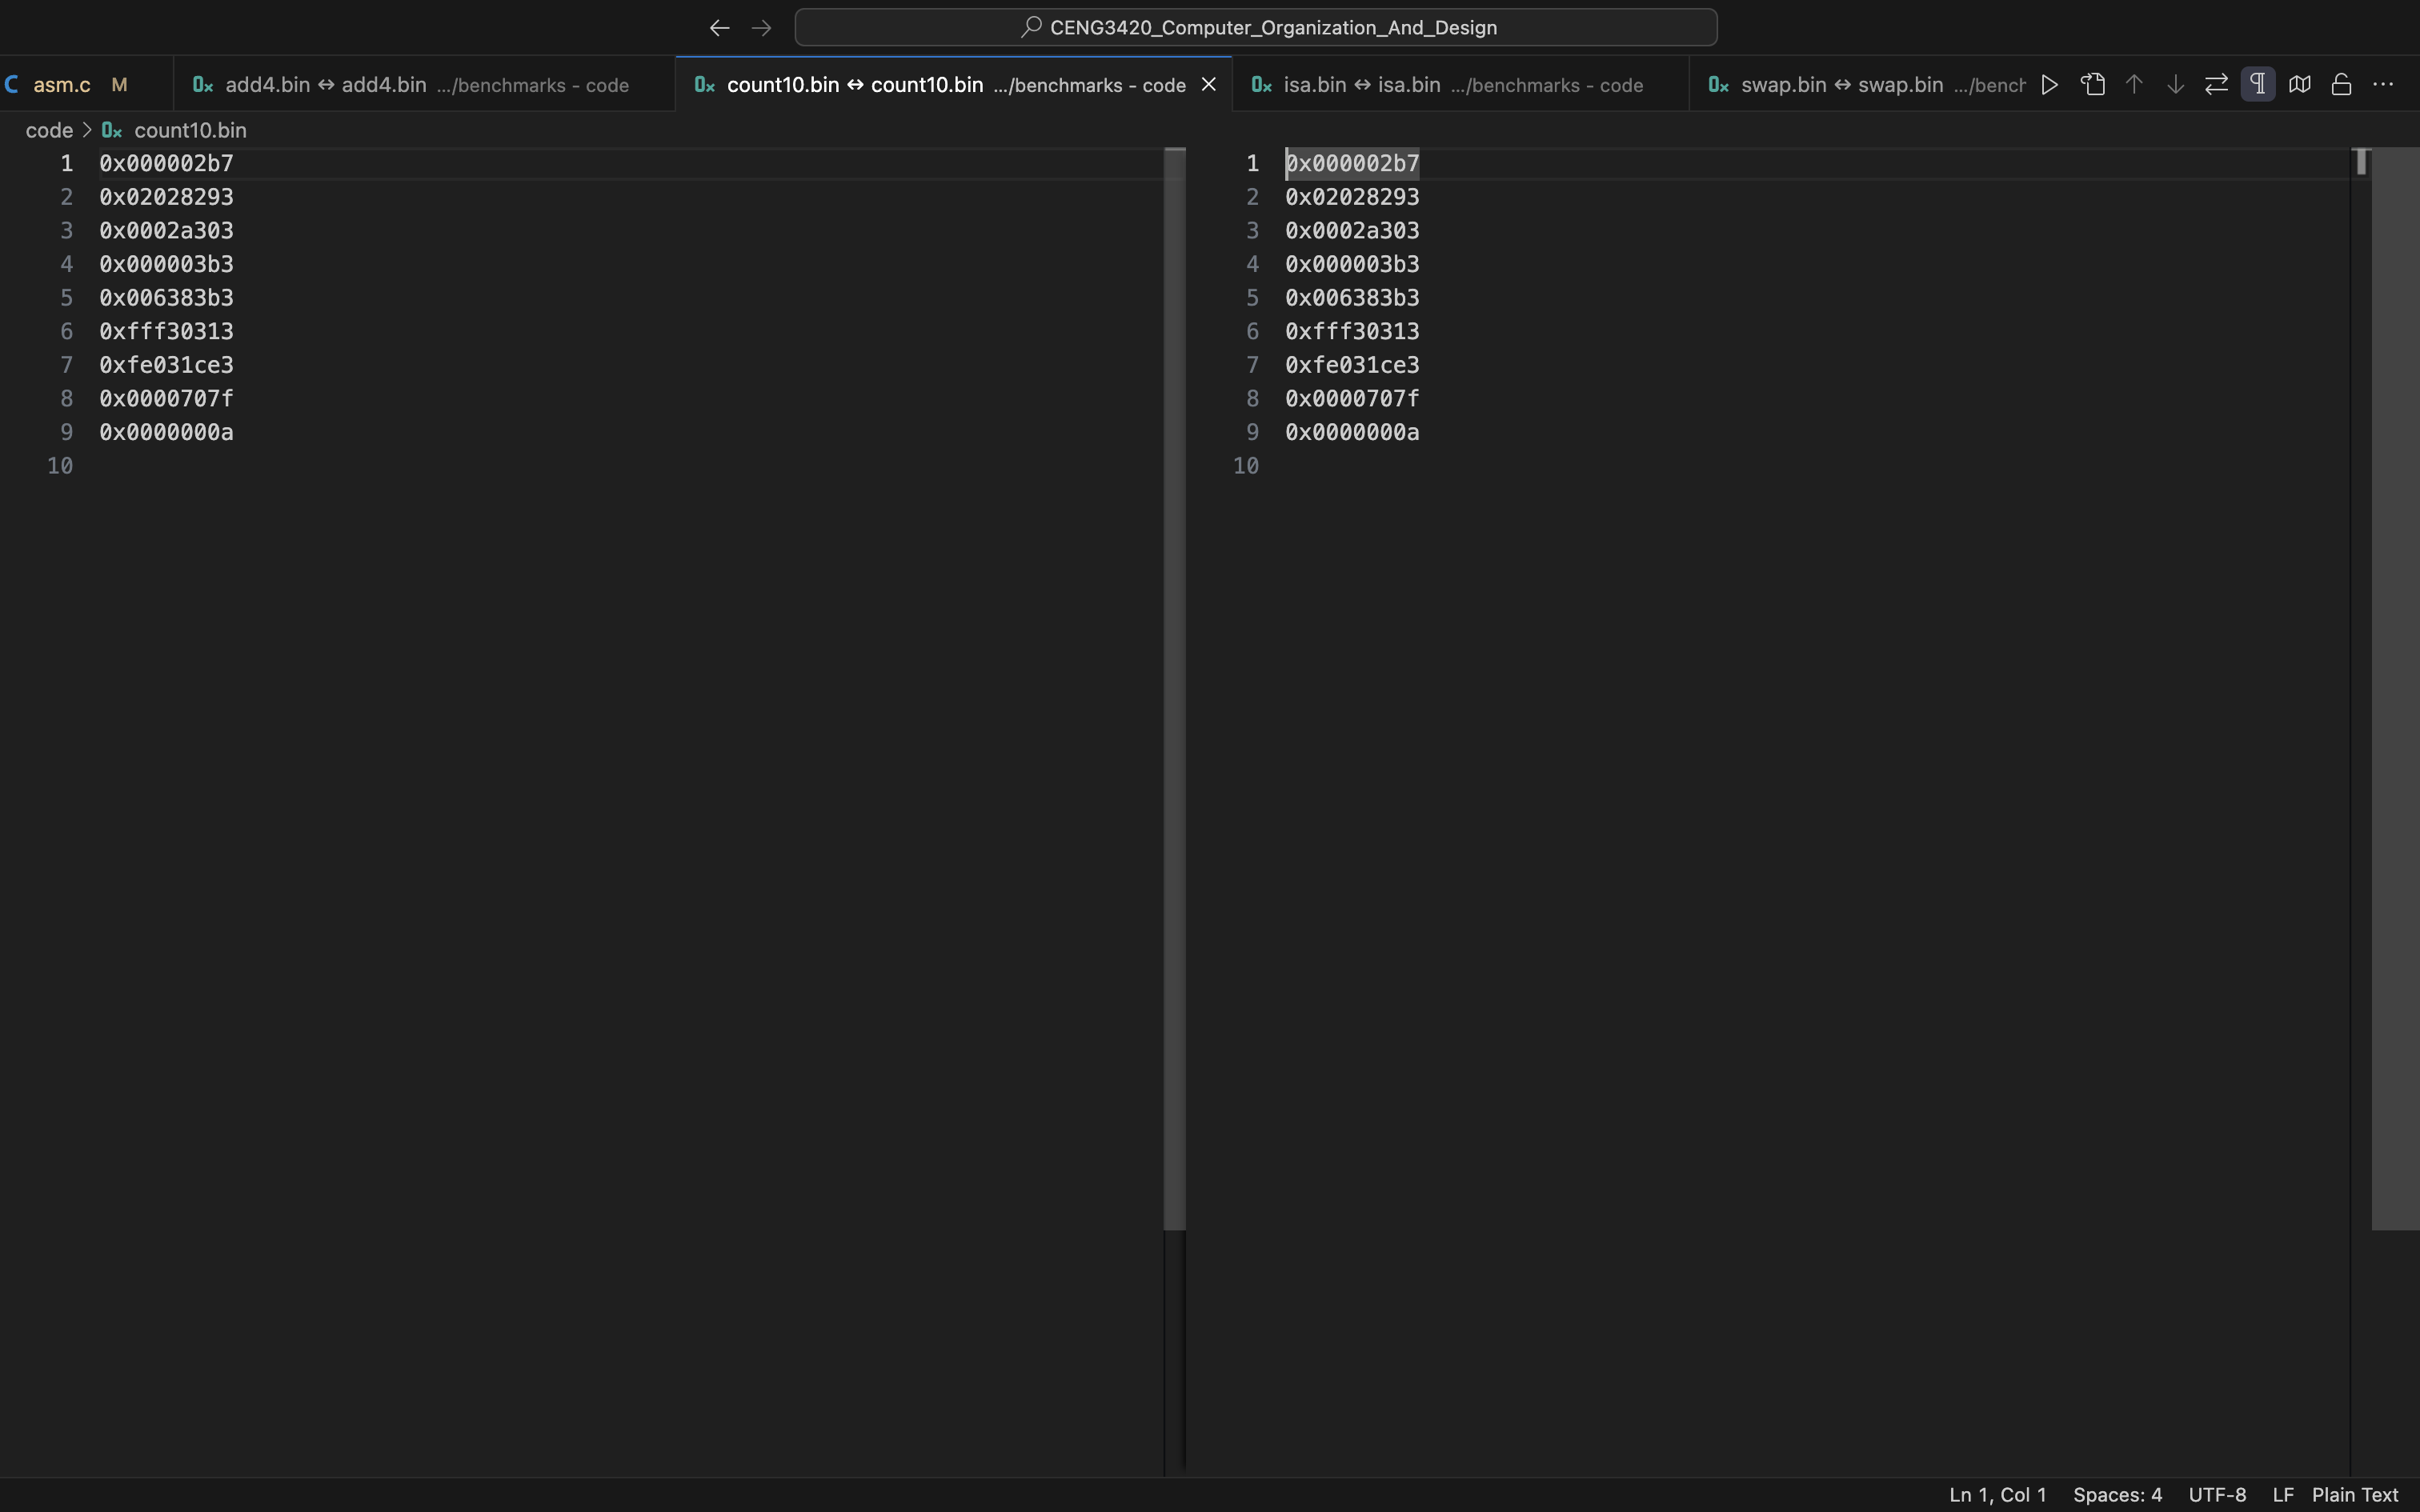
\includegraphics[width=1\linewidth]{../figs/count10.png}
\end{figure}

\begin{figure}[H]
    \caption{isa.bin}
    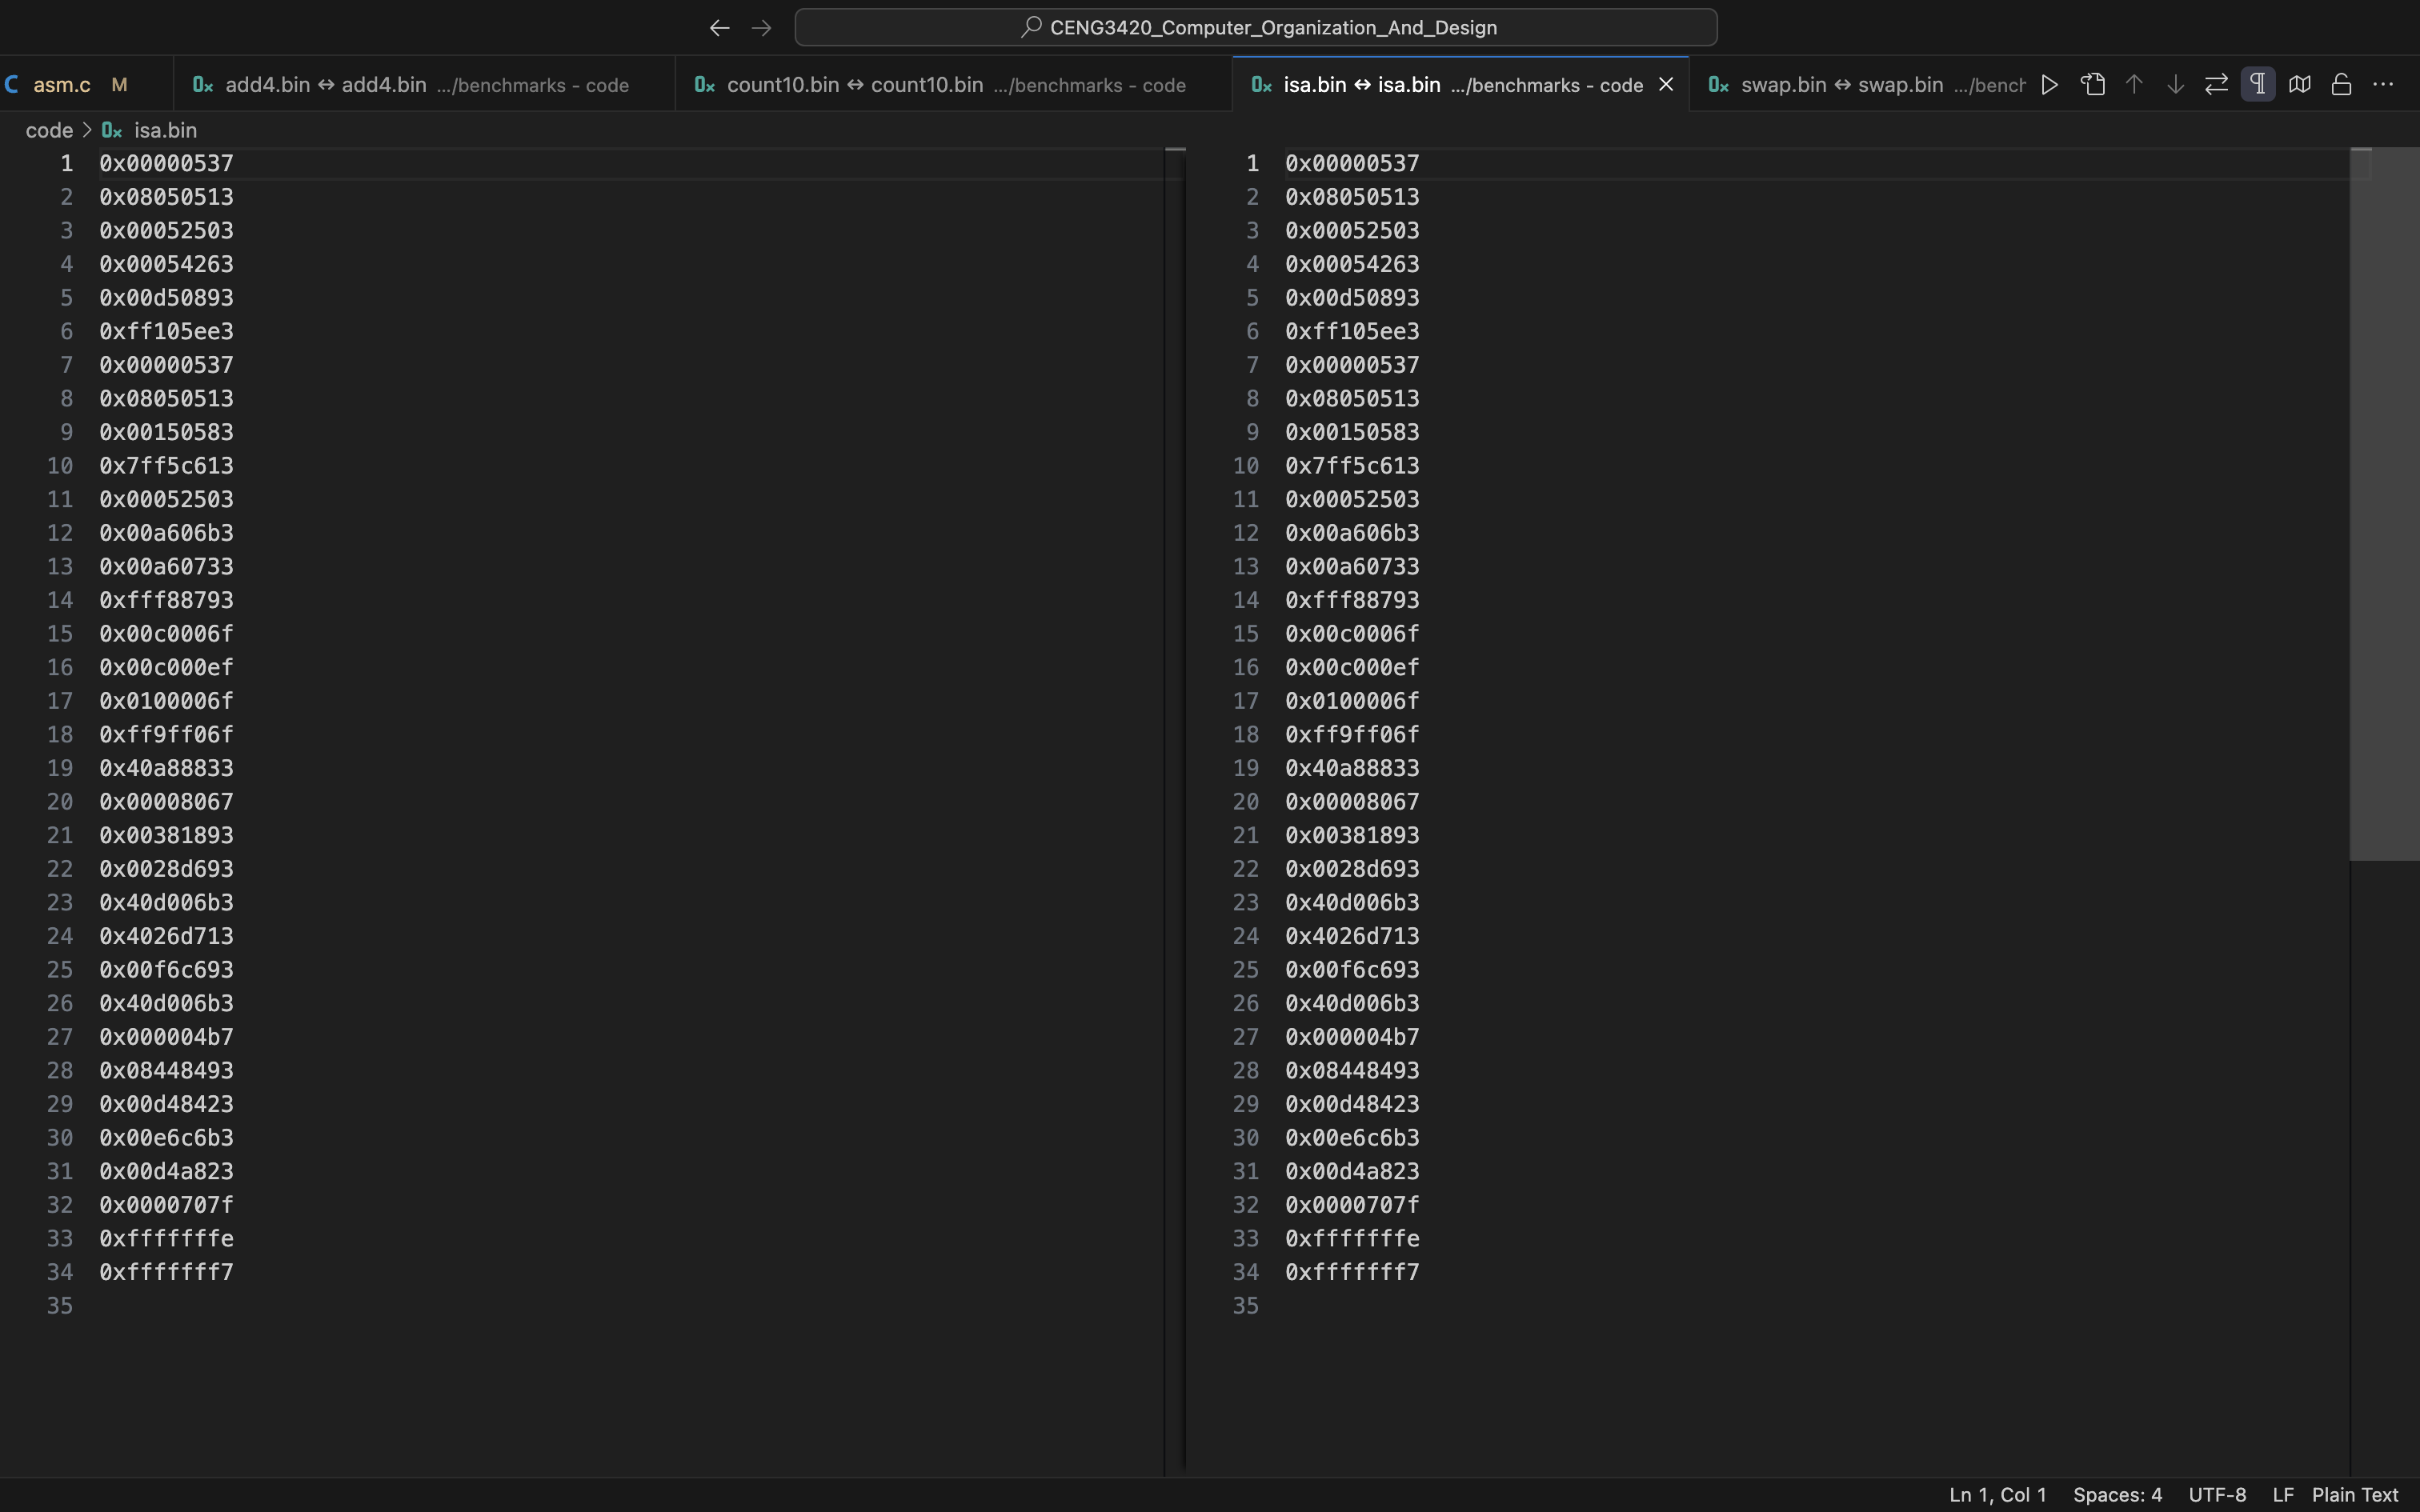
\includegraphics[width=1\linewidth]{../figs/isa.png}
\end{figure}

\begin{figure}[H]
    \caption{swap.bin}
    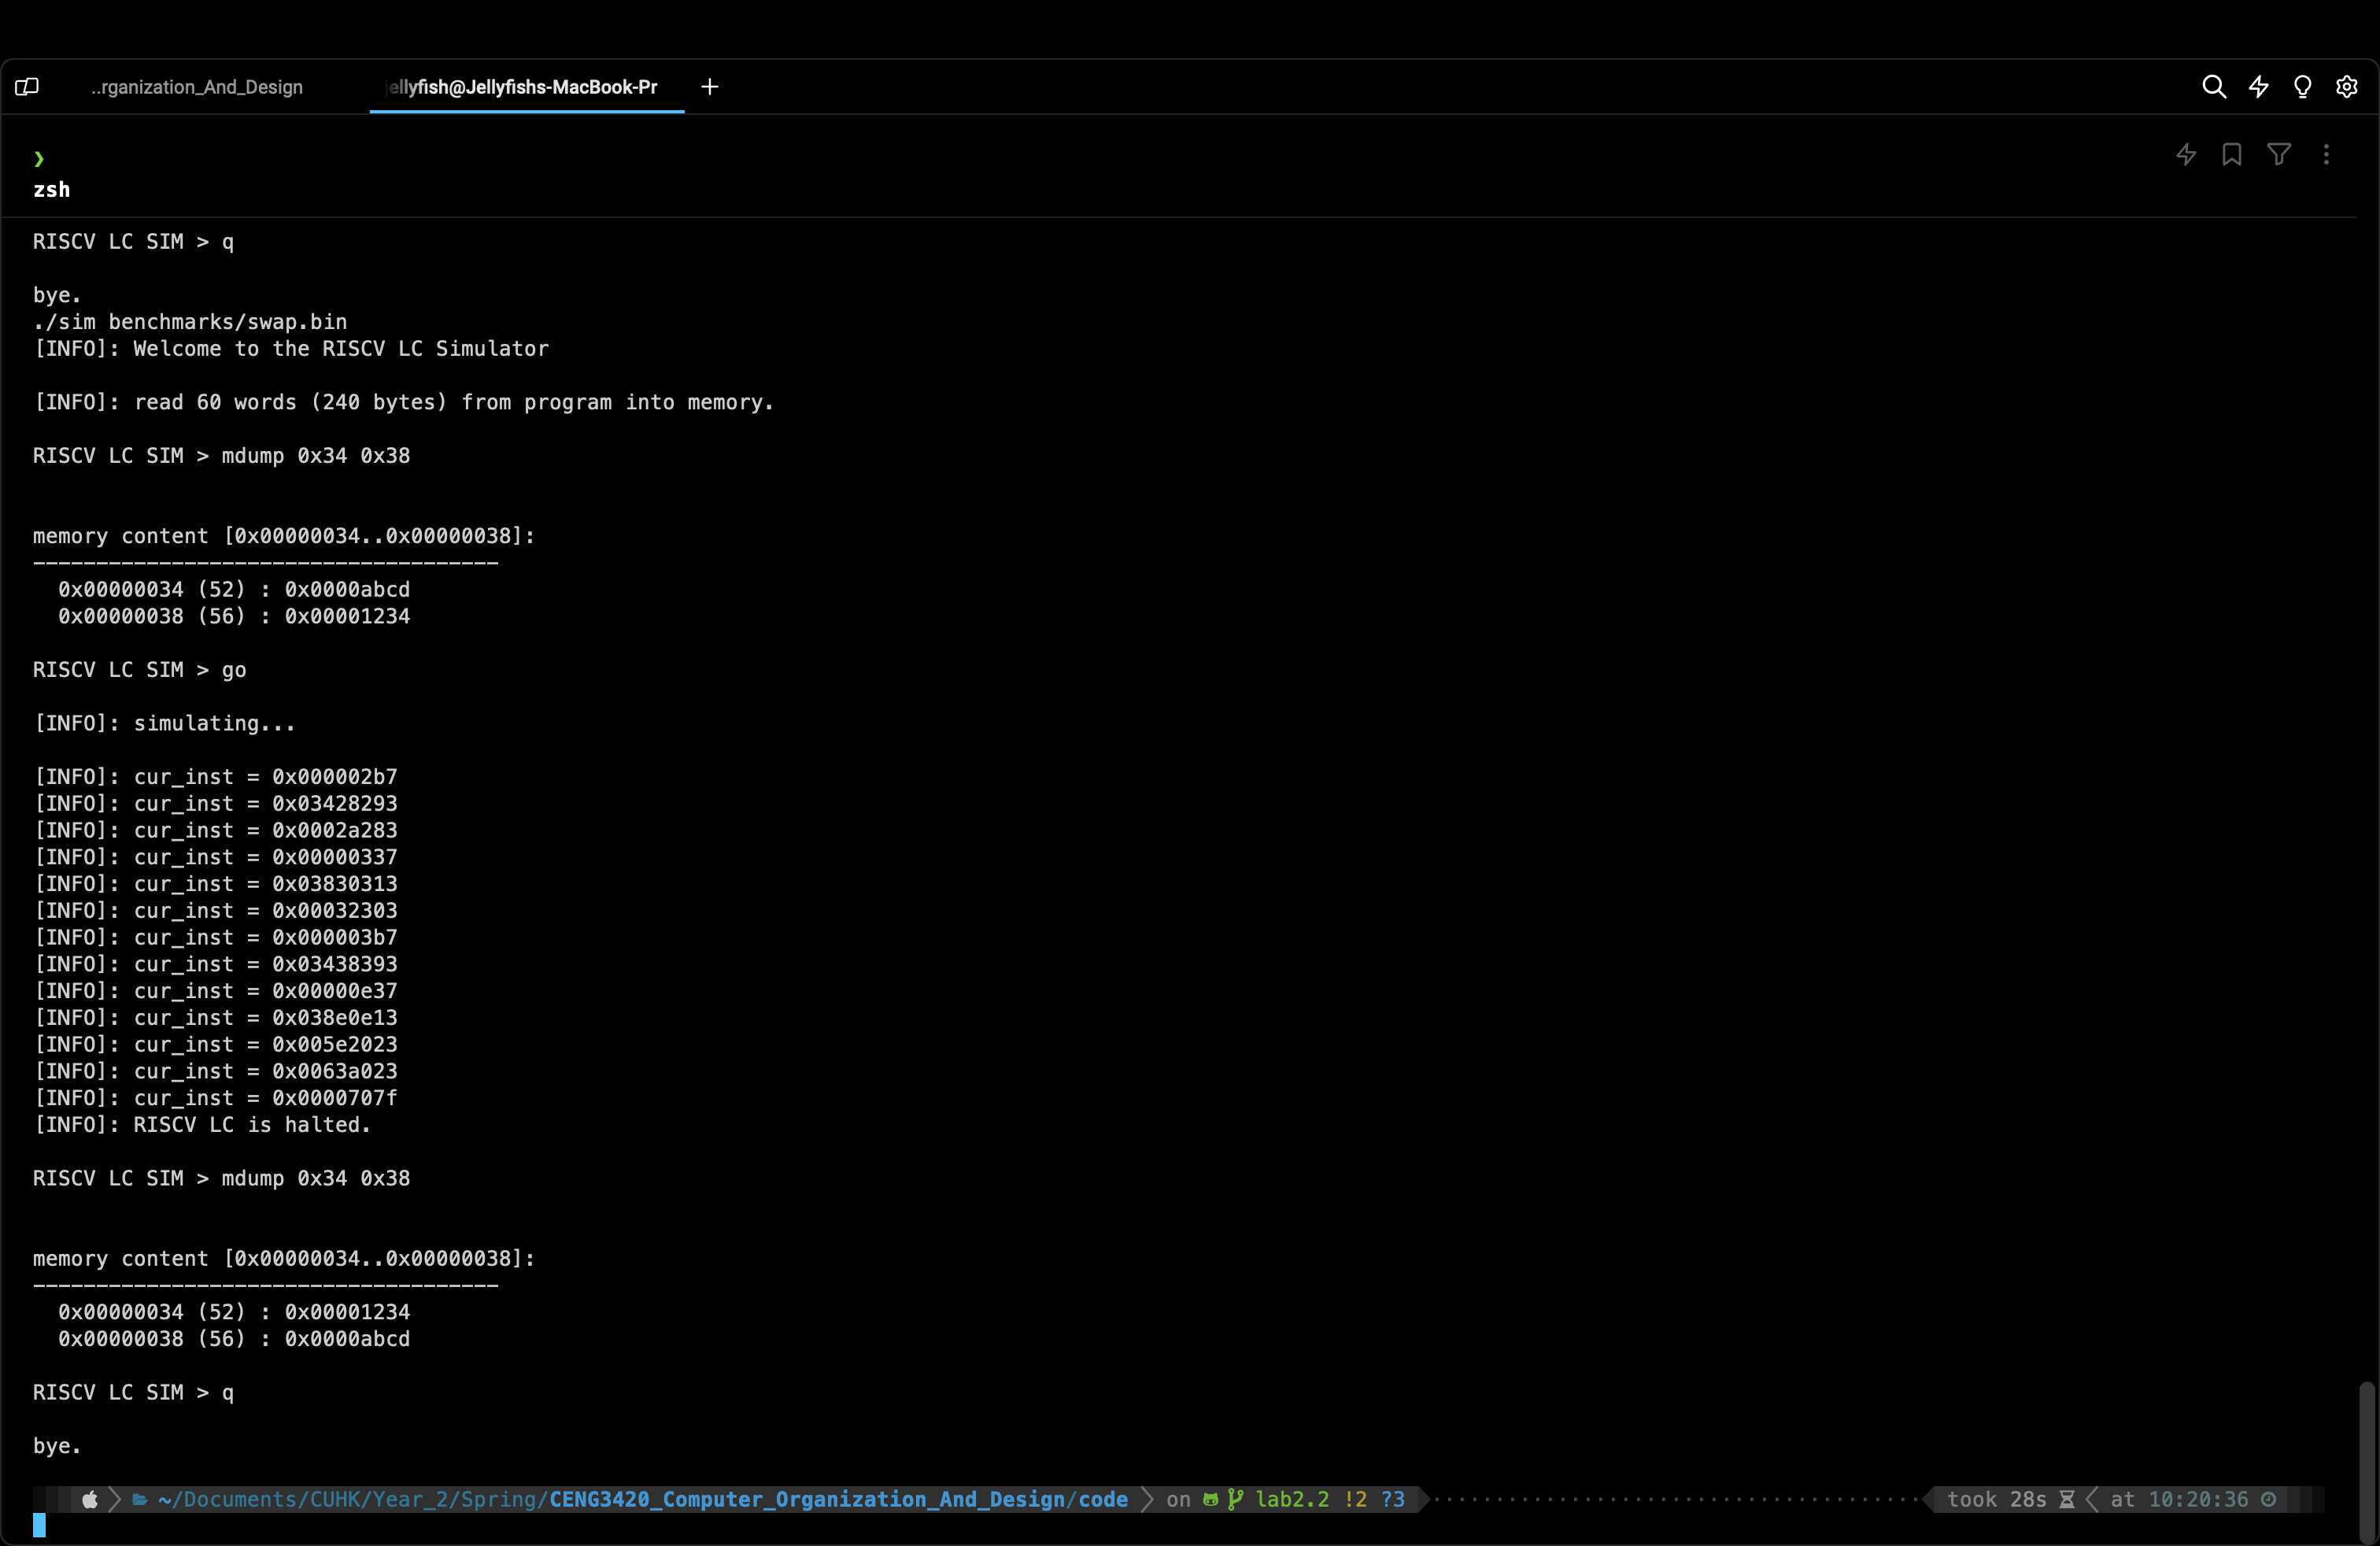
\includegraphics[width=1\linewidth]{../figs/swap.png}
\end{figure}

\end{document}
